%%=====================================================================================
%%
%%       Filename:  membrane.tex
%%
%%    Description:  
%%
%%        Version:  1.0
%%        Created:  05/05/2017
%%       Revision:  none
%%
%%         Author:  Dilawar Singh (), dilawars@ncbs.res.in
%%   Organization:  NCBS Bangalore
%%      Copyright:  Copyright (c) 2017, Dilawar Singh
%%
%%          Notes:  
%%                
%%=====================================================================================

\RequirePackage{luatex85}
\documentclass[crop,tikz]{standalone}
\usepackage{pgfplots}
\usetikzlibrary{shapes,arrows,arrows.meta}
\usetikzlibrary{calc,positioning,shadings}
\usetikzlibrary{decorations,decorations.shapes,decorations.markings}

% \ACTINDIMER{name}{pos}{radius}{rotation}
\newcommand\ACTINDIMER[4] {
    \pgfmathsetmacro{\r}{#3}
    \pgfmathsetmacro{\yshift}{\r*cos(#4)}
    \begin{scope}[ ]
        \edef\ballColor{white}
        \node[inner sep=0pt] (#1) at #2 { };
        \node[shading=ball,ball color=\ballColor,circle,minimum size=2*\r mm,inner sep=0] 
            (#1_up) at ([yshift=\yshift mm]#1) {};
        \node[shading=ball,ball color=\ballColor,circle,minimum size=2*\r mm,inner sep=0] 
            (#1_down) at ([yshift=-\yshift mm]#1) { };
    \end{scope}
}


\begin{document}
% membrane is made of lipid bilayer.
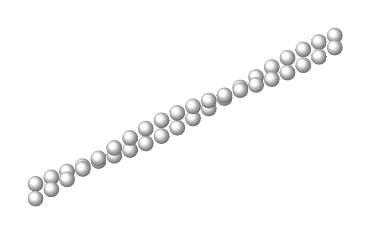
\begin{tikzpicture}[scale=1 , every node/.style={} ]
    % Draw helical path.
    \edef\r{1}        % Radius of actin.
    \foreach \i in {1,2,...,20}
    {
        \pgfmathsetmacro\x{\i*2*\r}
        \ACTINDIMER{a\i}{(\x mm,\i mm)}{1}{20*\i}
    }

    %% \path[ smooth
    %%         , decorate
    %%         , decoration={markings,
    %%             mark=between positions 0 and 1 step 0.05
    %%             with { 
    %%                 \node[minimum size=\r mm,shading=ball,circle] {}; 
    %%                 \node[minimum size=\r mm,shading=ball,circle,yshift=2*\r mm] {}; 
    %%             }
    %%             }
    %%     ] (2,0) -- (5,1) -- (10,0);

\end{tikzpicture}    

\end{document}
